% Preamble
\nonstopmode
\documentclass{beamer}
\usepackage{float}
% \usepackage[svgnames]{xcolor}
\usepackage[export]{adjustbox}
\usepackage{subcaption}
\usepackage{tikz}
\usepackage{pgfplots}
\usetikzlibrary{positioning}
\tikzstyle{block} = [rectangle, draw, text width=5em, text centered, rounded corners, minimum height=2em, font=\bf]
\tikzstyle{state} = [text width=9em, text centered]
\tikzstyle{blstate} = [rectangle, draw, text width=9em, text centered, minimum height=2em]

\AtBeginSection[]
{
  \begin{frame}
    \frametitle{Table of Contents}
    \tableofcontents[currentsection]
  \end{frame}
}

\definecolor{orange-red}{rgb}{1.0, 0.27, 0.0}

% Themes
	% \usetheme{umbc1} % good one
	% \usetheme{umbc2} % good one
	% \usetheme{Antibes} % good one
	% \usetheme{Warsaw} %<-- Well known blue theme
	% \usecolortheme{seahorse} % good one
	% \usetheme{Montpellier} % simple enough, but looks ok
	% \usetheme{default}

\usetheme[language=english,
		      titlepagelogo={Images/pyrforos},
		      notshowauthor=true,
          % assistantsupervisor=true,
		     ]{TorinoTh}

% \rel{Prof. Nektarios Koziris}
% \assistantsupervisor{Dr. Vangelis Koukis}
\institute{National Technical University of Athens}
\title[A Portable File Synchronisation Mechanism for a Cloud Storage Environment]{Design \& Implementation of a Portable File Synchronisation Mechanism for a Cloud Storage Environment}
\author{Vasilis Gerakaris}
\date{1/9/2015}

\begin{document}
\setsansfont[Mapping=TeX-text]{Linux Biolinum O}

\titlepageframe

\begin{tframe}
  \frametitle{Table of Contents}
    \tableofcontents%[pausesections]
\end{tframe}

\section{Introduction}
	\begin{tframe} \frametitle{Introduction}
		\highlightbf{File Synchronisation}: The process of updating files in two or more different locations, following certain rules. \\[5pt]
		\only<1>{ \framesubtitle{(i) - The problem}
      \highlightbf{Why is it needed?}
      \begin{itemize}
        \item Copying files between different computers
        \item Backups
      \end{itemize}

			\begin{block}{Important Qualities}
			\begin{adv}
				\item Needs to detect \& handle update conflicts/renames/deletions
				\item Needs to be reliable (no errors)
				\item Needs to be efficient
			\end{adv}
			\end{block}
		}

		\only<2>{ \framesubtitle{(i) - The problem (cont)}
      Software designed for that purpose already exists, namely:
      \begin{itemize}
        \item rsync
        \item ownCloud
        \item Dropbox
        \item Google Drive
      \end{itemize}
      We focus on a more specific aspect of the problem.
		}
	\end{tframe}

  \begin{tframe} \frametitle{Large Similar Files}
    \only<1>{ \framesubtitle{(i) - Definition}
      \highlightbf{What are they?}\\
      Files that satisfy the following two requirements:
      \begin{itemize}
        \item Are large in size (several GBs)
        \item Have a lot of their data in common
      \end{itemize}
      Examples: VM images, VM snapshots\\[5pt]
      \highlightbf{Why are they important?}

      Many VMs are being used on cloud service providers (Amazon AWS, \textasciitilde okeanos, etc) and there should be a way to efficiently synchronise their images and snapshots.
    }
    \only<2>{ \framesubtitle{(ii) - Definition (cont)}
      \begin{figure}[!htpb]
        \centering
        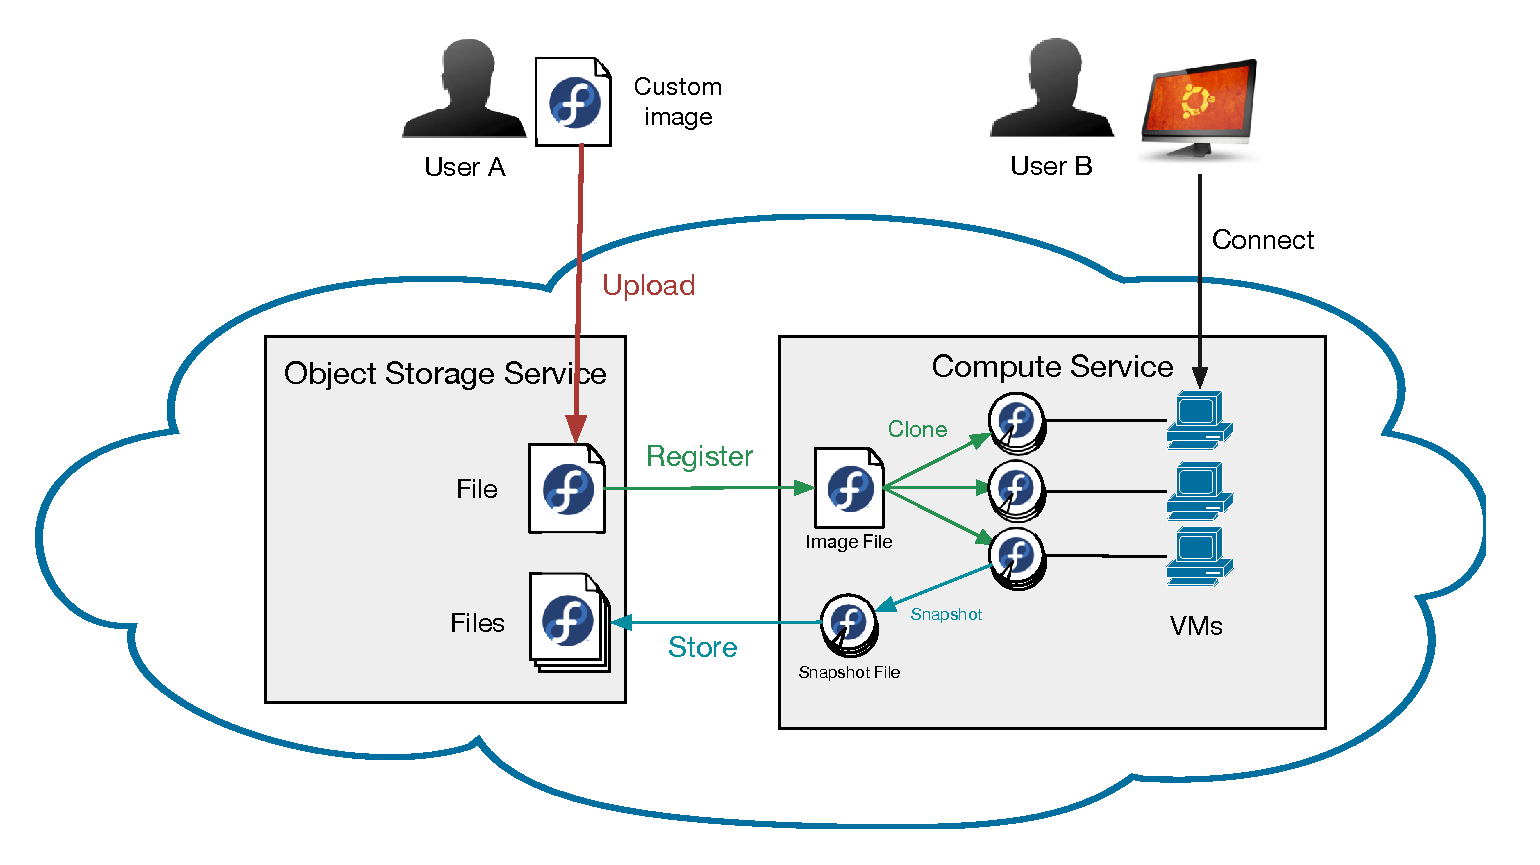
\includegraphics[width=0.85\textwidth]{Images/cloud}
      \end{figure}
    }
    \only<3>{ \framesubtitle{(iii) - Definition (cont)}
      \begin{figure}[!htpb]
        \centering
        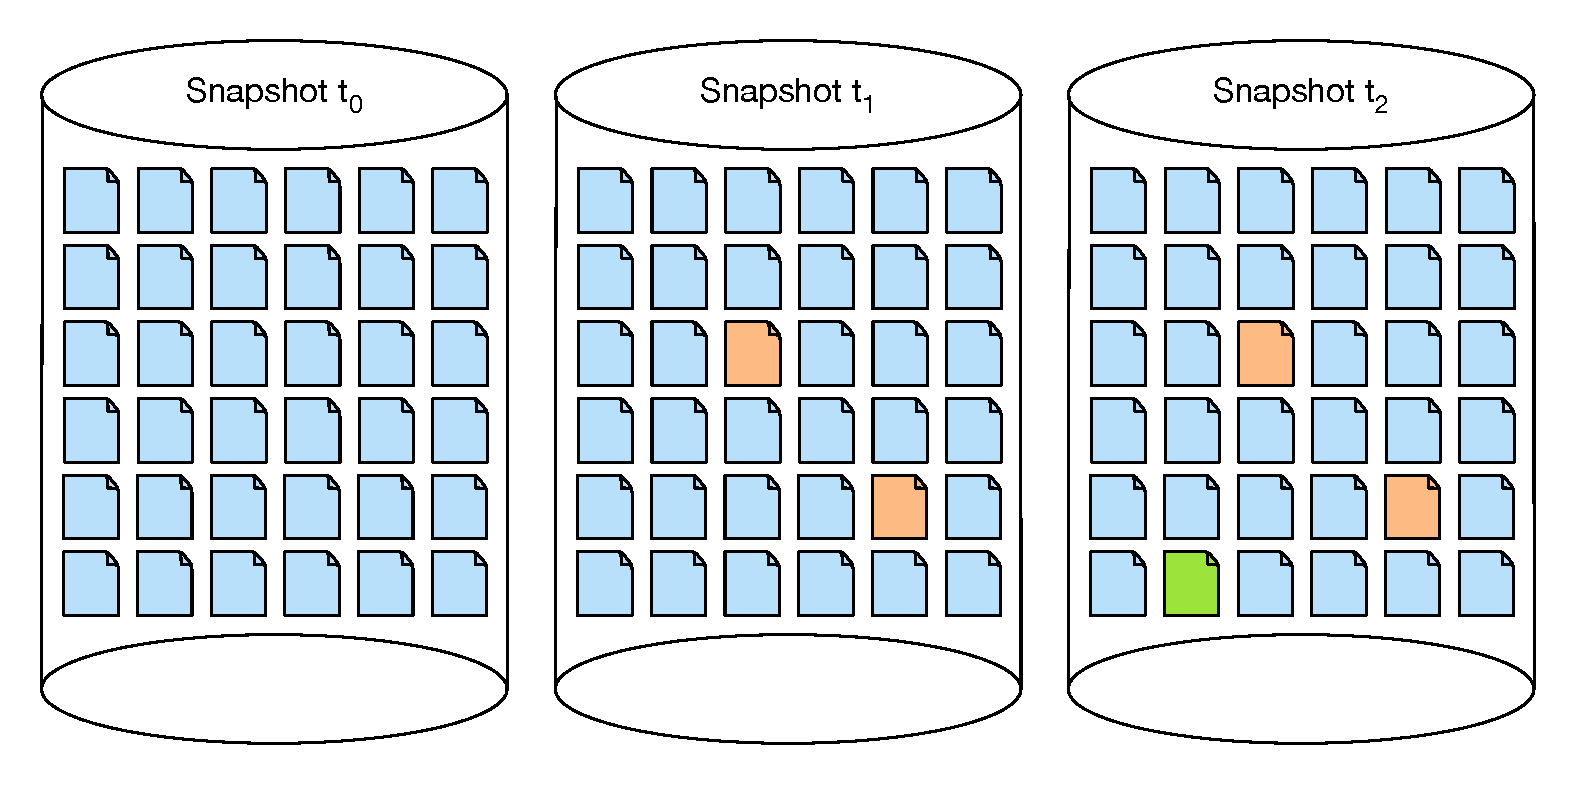
\includegraphics[width=0.85\textwidth]{Images/LSF}
      \end{figure}
      \alert{We can use these similarities to optimise the synchronisation!}
    }
  \end{tframe}

\section{Design \& Implementation}
	\subsection{Syncing algorithm}
	\begin{tframe} \frametitle{Syncing algorithm}
		\only<1>{ \framesubtitle{(i) - Modification detection}
			\highlightbf{Modification detection}: Comparison of hash digests
      \begin{adv}
      \item Reliable
      \end{adv}
      \begin{disadv}
      \item Very slow, especially on large files
      \end{disadv}
      Faster alternative: Use last modification time as an indicator.\\[5pt]
      \highlightbf{Why we need history data:}\\
      Need to know what to do in the following cases:
      \begin{itemize}
        \item File exists on both locations and is different
        \item File exists on A but not on B (or vice-versa)
      \end{itemize}
		}

		\only<2>{ \framesubtitle{(ii) - Initial algorithm}
	    \begin{table}[H]
      \centering
      \begin{adjustbox}{max width=0.7\textwidth, center}
      \begin{subtable}{\textwidth}
        \centering
        \begin{tabular}{|l|l|l|}
          \hline \textbf{Time $T_1$} & \textbf{Time $T_2$} & \textbf{Change}\\ \hline \hline
           Does not Exist & Exists & Created \\ \hline
           Exists & Does not Exist & Deleted \\ \hline
           Exists (ETag = J) & Exists (Etag = J) & No Change \\ \hline
           Exists (Etag = J) & Exists (Etag = K) & Modified \\ \hline
        \end{tabular}
        \caption{File change detection between two points in time}
      \end{subtable}
      \end{adjustbox}
      \begin{adjustbox}{max width=0.7\textwidth, center}
      \begin{subtable}{\textwidth}
        \centering
        \begin{tabular}{|l|l|l|}
          \hline \textbf{File replica A} & \textbf{File replica B} & \textbf{Action} \\ \hline \hline
           No Change & No Change & No Action \\ \hline
           Created (ETag = J) & Created (Etag = J) & No Action \\ \hline
           Created (ETag = J) & Created (Etag = K) & \emph{Merge$^*$} \\ \hline
           Deleted & Deleted & No Action \\ \hline
           Deleted & No Change & Delete B \\ \hline
           Modified & No Change & Update B \\ \hline
           Modified (ETag = J) & Modified (ETag = K) & \emph{Merge$^*$} \\ \hline
        \end{tabular}
        \caption{Syncing actions based on file states}
      \end{subtable}
      \end{adjustbox}
      \end{table}
		}

    \only<3>{ \framesubtitle{(iii) - What we propose}
      \highlightbf{Limitations}\\
      \begin{disadv}
        \item Can't detect renames (or worse, renames \& modifications)
      \end{disadv}
      \highlightbf{Our solution for syncing with a central metadata server}\\
      \begin{itemize}
        \item Store the metadata of all files, as they were during the last successful sync on a local state database (StateDB).
        \item Reconcile local directory replicas (Local) and remote server replicas (Remote) in three steps:
        \begin{enumerate}
          \item Detect updates from Local Directory
          \item Detect updates from StateDB
          \item Detect updates from Remote Directory
        \end{enumerate}
        \item FCFS updates on conflicts, with conflicting copies being renamed.
      \end{itemize}
    }
	\end{tframe}
  \begin{tframe} \frametitle{3-step synchronisation}
    \only<1>{ \framesubtitle{(i) - Updates from Local Directory}
      \begin{figure}[H]
        \centering
        \begin{adjustbox}{max width=.8\textwidth, center}
        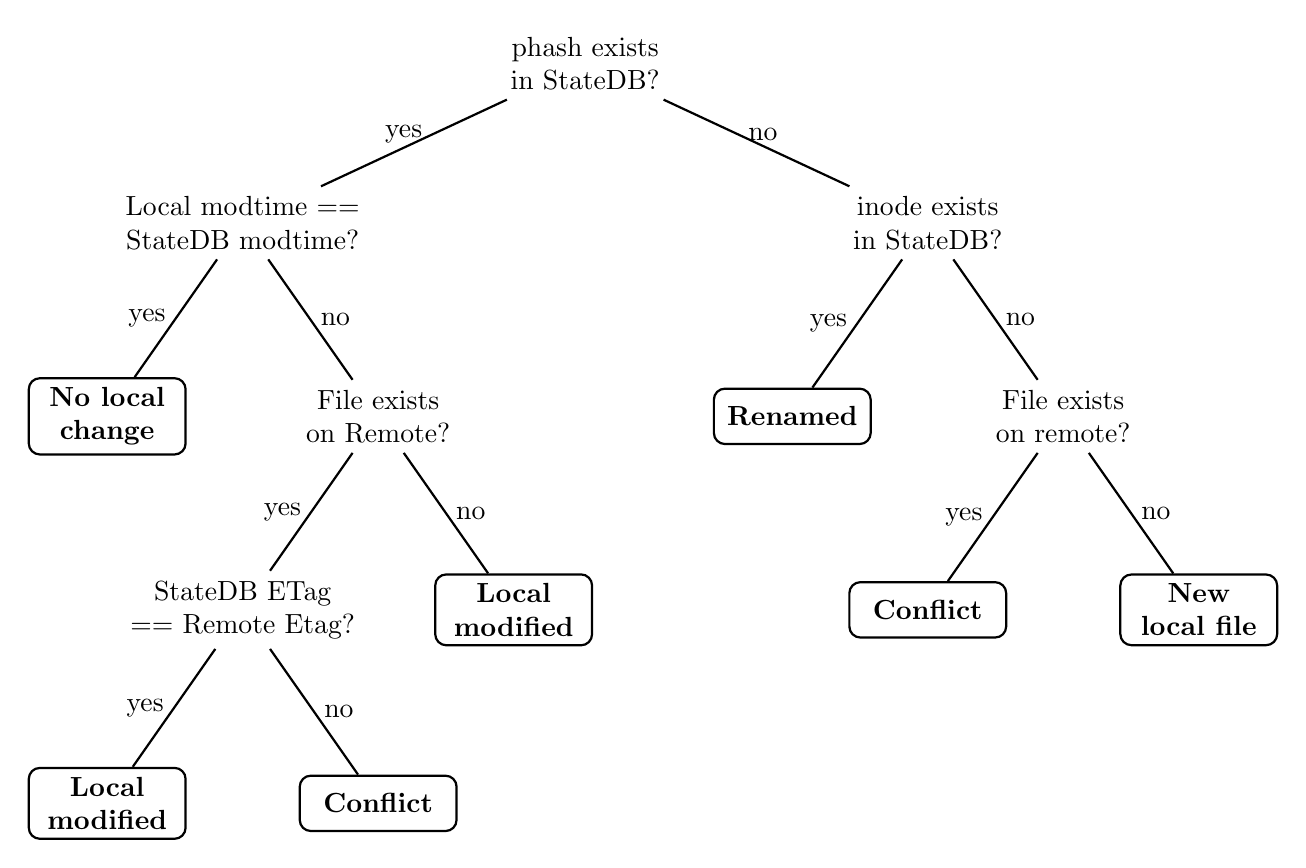
\begin{tikzpicture}[thick]
        \newdimen\nodeDist
        \nodeDist=30mm

          \node [state] (A) {phash exists in StateDB?};
          \path (A) ++(-155:1.6\nodeDist) node [state] (B) {Local modtime == StateDB modtime?};
          \path (A) ++(-25:1.6\nodeDist) node [state] (C) {inode exists in StateDB?};

          \path (B) ++(-125:\nodeDist) node [block] (B-1) {No local change};
          \path (B) ++(-55:\nodeDist) node [state] (B-2) {File exists on Remote?};
          \path (B-2) ++(-125:\nodeDist) node [state] (B-2-1) {StateDB ETag == Remote Etag?};
          \path (B-2) ++(-55:\nodeDist) node [block] (B-2-2) {Local modified};
          \path (B-2-1) ++(-125:\nodeDist) node [block] (B-2-1-1) {Local modified};
          \path (B-2-1) ++(-55:\nodeDist) node [block] (B-2-1-2) {Conflict};

          \path (C) ++(-125:\nodeDist) node [block] (C-1) {Renamed};
          \path (C) ++(-55:\nodeDist) node [state] (C-2) {File exists on remote?};
          \path (C-2) ++(-125:\nodeDist) node [block] (C-2-1) {Conflict};
          \path (C-2) ++(-55:\nodeDist) node [block] (C-2-2) {New local file};


          \draw (A) -- (B) node [left,pos=0.4] {yes};
          \draw (A) -- (C) node [right,pos=0.4] {no};
          \draw (B) -- (B-1) node [left,pos=0.5] {yes};
          \draw (B) -- (B-2) node [right,pos=0.5] {no};
          \draw (B-2) -- (B-2-1) node [left,pos=0.5] {yes};
          \draw (B-2) -- (B-2-2) node [right,pos=0.5] {no};
          \draw (B-2-1) -- (B-2-1-1) node [left,pos=0.5] {yes};
          \draw (B-2-1) -- (B-2-1-2) node [right,pos=0.5] {no};
          \draw (C) -- (C-1) node [left,pos=0.5] {yes};
          \draw (C) -- (C-2) node [right,pos=0.5] {no};
          \draw (C-2) -- (C-2-1) node [left,pos=0.5] {yes};
          \draw (C-2) -- (C-2-2) node [right,pos=0.5] {no};
        \end{tikzpicture}
        \end{adjustbox}
      \end{figure}
    }
    \only<2>{ \framesubtitle{(ii) - Updates from StateDB}
      \begin{figure}[H]
        \centering
        \begin{adjustbox}{max width=.85\textwidth, center}
        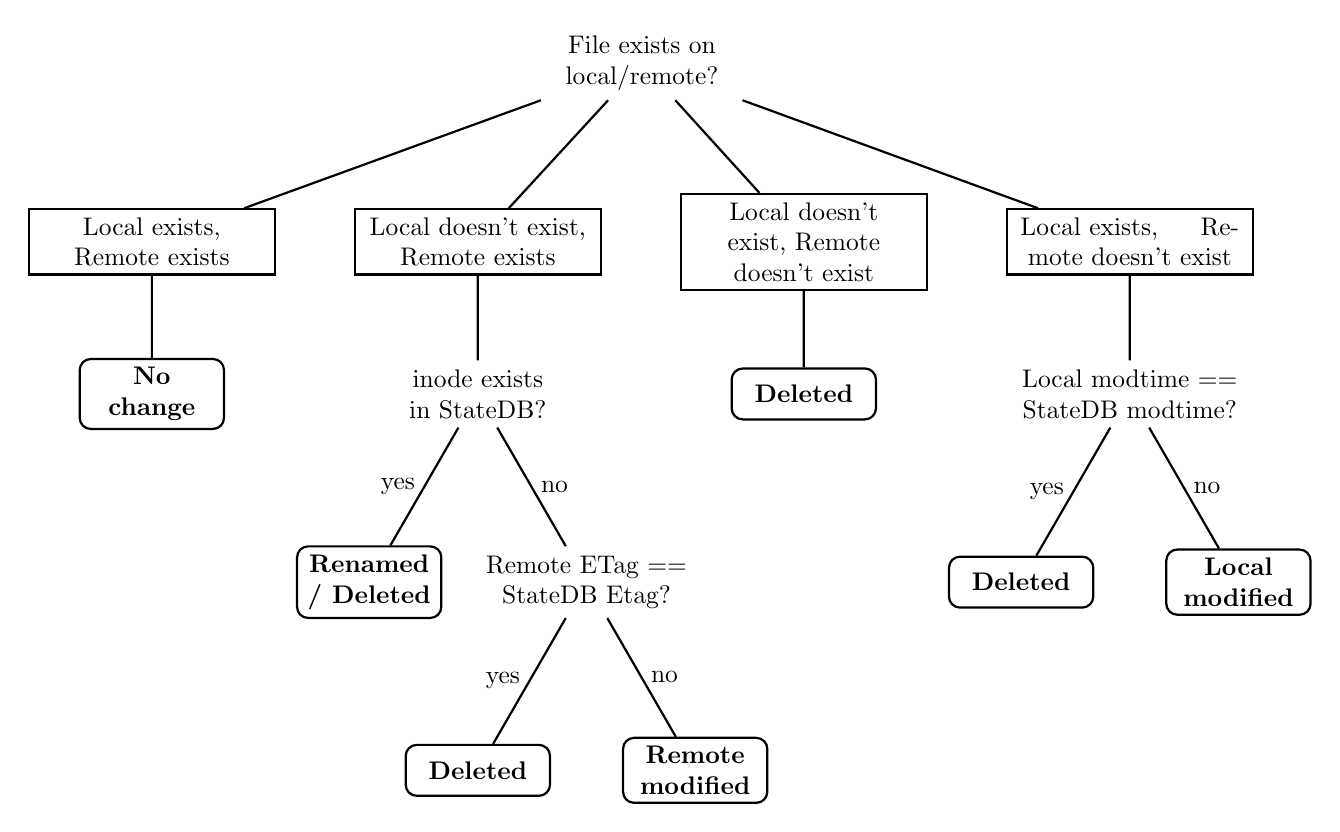
\begin{tikzpicture}[scale=0.92, thick, every node/.style={transform shape}]
        \newdimen\nodeDist
        \nodeDist=30mm

          \node [state] (S) {File exists on local/remote?};
          \path (S) ++(-160:2.4\nodeDist) node [blstate] (A) {Local exists, Remote exists};
          \path (A) ++(0:1.5\nodeDist) node [blstate] (C) {Local doesn't exist, Remote exists};
          \path (C) ++(0:1.5\nodeDist) node [blstate] (B) {Local doesn't exist, Remote doesn't exist};
          \path (B) ++(0:1.5\nodeDist) node [blstate] (D) {Local exists, \hspace{1em} Remote doesn't exist};
          \path (A) ++(-90:0.7\nodeDist) node [block] (AA) {No change};
          \path (B) ++(-90:0.7\nodeDist) node [block] (BB) {Deleted};
          \path (C) ++(-90:0.7\nodeDist) node [state] (CC) {inode exists in StateDB?};
          \path (CC) ++(-120:\nodeDist) node [block] (CC-1) {Renamed / Deleted};
          \path (CC) ++(-60:\nodeDist) node [state] (CC-2) {Remote ETag == StateDB Etag?};
          \path (CC-2) ++(-120:\nodeDist) node [block] (CC-2-1) {Deleted};
          \path (CC-2) ++(-60:\nodeDist) node [block] (CC-2-2) {Remote modified};
          \path (D) ++(-90:0.7\nodeDist) node [state] (DD) {Local modtime == StateDB modtime?};
          \path (DD) ++(-120:\nodeDist) node [block] (DD-1) {Deleted};
          \path (DD) ++(-60:\nodeDist) node [block] (DD-2) {Local modified};


          \draw (S) -- (A);
          \draw (S) -- (B);
          \draw (S) -- (C);
          \draw (S) -- (D);
          \draw (A) -- (AA);
          \draw (B) -- (BB);
          \draw (C) -- (CC);
          \draw (D) -- (DD);
          \draw (CC) -- (CC-1) node [left,pos=0.5] {yes};
          \draw (CC) -- (CC-2) node [right,pos=0.5] {no};
          \draw (CC-2) -- (CC-2-1) node [left,pos=0.5] {yes};
          \draw (CC-2) -- (CC-2-2) node [right,pos=0.5] {no};
          \draw (DD) -- (DD-1) node [left,pos=0.5] {yes};
          \draw (DD) -- (DD-2) node [right,pos=0.5] {no};
        \end{tikzpicture}
        \end{adjustbox}
      \end{figure}
    }
    \only<3>{ \framesubtitle{(iii) - Updates from Remote Directory}
      \begin{figure}[H]
        \centering
        \begin{adjustbox}{max width=.45\textwidth, center}
        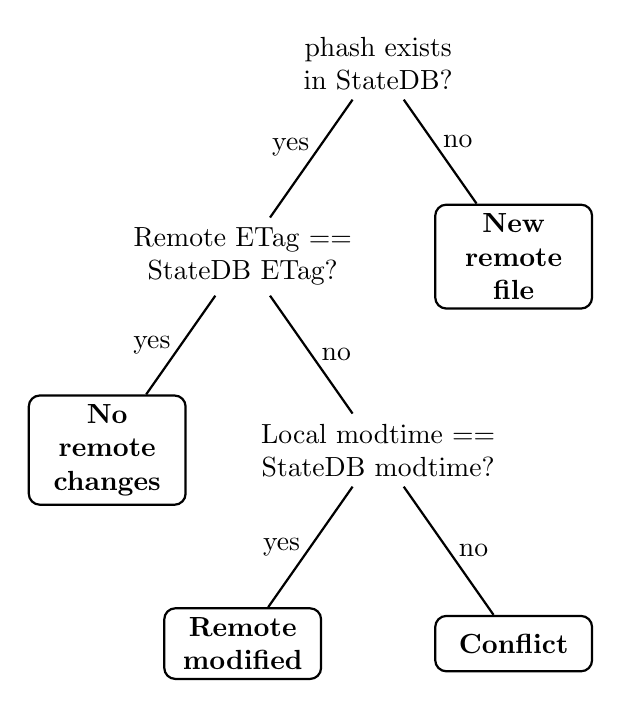
\begin{tikzpicture}[thick]
        \newdimen\nodeDist
        \nodeDist=30mm

          \node [state] (A) {phash exists in StateDB?};
          \path (A) ++(-125:\nodeDist) node [state] (B) {Remote ETag == StateDB ETag?};
          \path (A) ++(-55:\nodeDist) node [block] (C) {New remote file};

          \path (B) ++(-125:\nodeDist) node [block] (B-1) {No remote changes};
          \path (B) ++(-55:\nodeDist) node [state] (B-2) {Local modtime == StateDB modtime?};
          \path (B-2) ++(-125:\nodeDist) node [block] (B-2-1) {Remote modified};
          \path (B-2) ++(-55:\nodeDist) node [block] (B-2-2) {Conflict};

          \draw (A) -- (B) node [left,pos=0.4] {yes};
          \draw (A) -- (C) node [right,pos=0.4] {no};
          \draw (B) -- (B-1) node [left,pos=0.5] {yes};
          \draw (B) -- (B-2) node [right,pos=0.5] {no};
          \draw (B-2) -- (B-2-1) node [left,pos=0.5] {yes};
          \draw (B-2) -- (B-2-2) node [right,pos=0.5] {no};
        \end{tikzpicture}
        \end{adjustbox}
      \end{figure}
    }
  \end{tframe}

	\subsection{Core Classes / API}
  \begin{tframe} \frametitle{Core Classes / API}
    What we have done:
    \begin{itemize}
      \item Built a cross-platform framework in Python that can be used to synchronise files with any cloud storage service, as long as some API functions are implemented.
      \item Created abstract classes for representations of files, filesystem directories and cloud storage services.
      \item Implemented a class that uses the Synnefo (Pithos) API as an example.
      \item Created a proof-of-concept application that syncs a local directory with the Pithos+ service offered by \textasciitilde okeanos.
    \end{itemize}
  \end{tframe}
	\begin{tframe} \frametitle{Core Classes / API}
		\only<1>{ \framesubtitle{(i) - FileStat}
    \begin{minipage}{0.3\textwidth}
      \centering
      \begin{figure}[!htpb]
        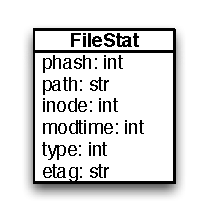
\includegraphics[width=\textwidth]{Images/FileStat.eps}
      \end{figure}
    \end{minipage}
    \begin{minipage}{0.65\textwidth}
      The core class used in this framework to \mbox{represent} file objects
      \begin{itemize}
        \item \textbf{phash}: The (integer) hash digest of the relative path string. It is used for fast indexing in the StateDB. Assumed unique for each file path.
        \item \textbf{etag}: The ETag (sha-256 digest) of the file. Assumed unique for each file version.
      \end{itemize}
    \end{minipage}
		}
		\only<2>{ \framesubtitle{(ii) - LocalDirectory}
      \begin{figure}[!htpb]
        \centering
        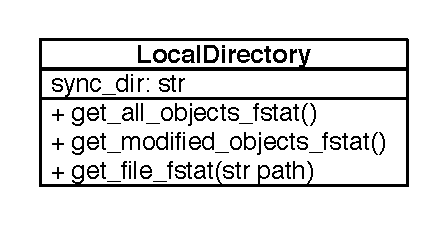
\includegraphics[width=0.45\textwidth]{Images/LocalDir.eps}
      \end{figure}
      \small{
      \begin{itemize}
        \item \textbf{get\_all\_objects\_fstat}: Returns all local files' metadata as FileStat objects.
        \item \textbf{get\_modified\_objects\_fstat}: Return file metadata only for the files that were modified since the last sync.
        \item \textbf{get\_file\_fstat}: Returns the FileStat object for the file \emph{path} if it exists, else returns \emph{None}.
      \end{itemize}
      }
		}
		\only<3>{ \framesubtitle{(iii) - CloudClient}
	    \begin{figure}[!htpb]
        \centering
        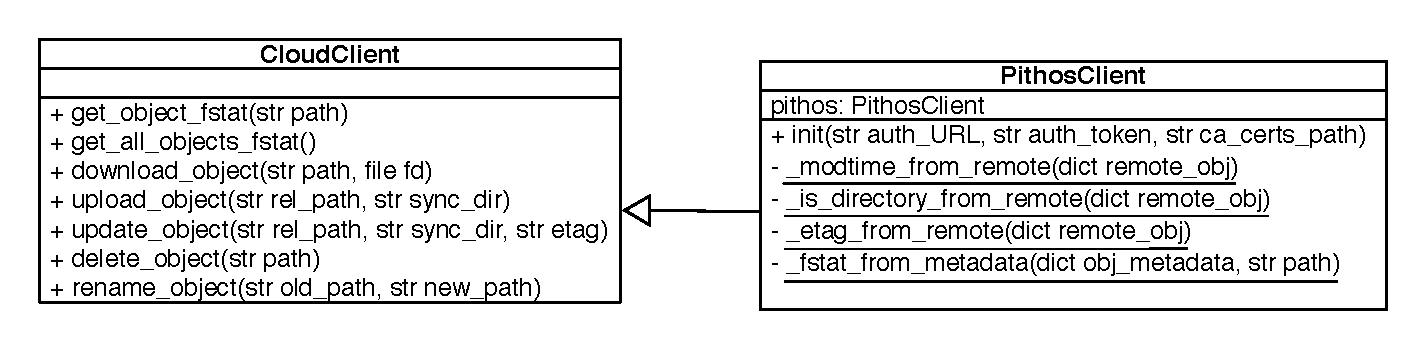
\includegraphics[width=1.05\textwidth]{Images/CloudClient.eps}
      \end{figure}
      Closely resembles the OpenStack API (used by synnefo as well).\\
      To properly handle race conditions:\\
      \textbf{upload\_object()} is used for new files\\
      \textbf{update\_object()} is used for existing files.
		}
	\end{tframe}

\section{Optimisations}
	\subsection{Request Queuing}
  	\begin{tframe} \frametitle{Optimisation: Request Queuing}
  		\only<1>{ \framesubtitle{(i) - Description}
  			\begin{block}<1->{Multiple requests are slow!}
          \begin{adv}
            \item Batch them wherever possible (\alert{get\_all\_objects\_fstat()})
            \item Use threads and queues to send requests without waiting for others to complete.
          \end{adv}
        \end{block}
        \begin{disadv}
          \item Need to wait for completion of all threads at a step of the sync algorithm before proceding to the next.
          \begin{itemize}
            \item Can be further optimised using a locking mechanism
          \end{itemize}
        \end{disadv}
  		}
  		\only<2>{ \framesubtitle{(ii) - Benchmark results}
  			\begin{table}
          \begin{subtable}{\textwidth}
          \centering
          \begin{adjustbox}{max width=\textwidth, center}
            \begin{tabular}{c|*{12}{c|}}
              \cline{2-12}
              & \multicolumn{11}{ |c| }{\textbf{\# of threads}} \\ \cline{2-12}
              & \textbf{0} & \textbf{1} & \textbf{2} & \textbf{4} & \textbf{8} & \textbf{12} & \textbf{16} & \textbf{20} & \textbf{24} & \textbf{28} & \textbf{32} \\ \cline{1-12}
              \multicolumn{1}{ |c| }{\textbf{time (s)}} & 92.55 & 91.51 & 48.33 & 33.42 & 29.79 & 29.80 & 30.85 & 30.79 & 30.95 & 30.68 & 31.23 \\ \cline{1-12}
              \multicolumn{1}{ |c| }{\textbf{speedup (\%)}} & N/A & 1.51 & 47.78 &  63.89 & 67.81 & 67.80 & 66.67 & 66.73 & 66.56 & 66.85 & 66.25 \\ \cline{1-12}
            \end{tabular}
          \end{adjustbox}
          \caption{Upload speedup by queuing, relative to \# of threads}
          \end{subtable}
          \begin{subtable}{\textwidth}
          \centering
            \begin{adjustbox}{max width=.55\textwidth, center}
            \begin{tabular}{c|*{4}{c|}}
              \cline{2-4}
              & \multicolumn{3}{ |c| }{\textbf{File Size}} \\ \cline{2-4}
              & \textbf{150 B} & \textbf{150 KB} & \textbf{1.5 MB} \\ \cline{1-4}
              \multicolumn{1}{ |c| }{\textbf{Sequential upload time (s)}} & 92.55 & 153.32 & 636.48 \\ \cline{1-4}
              \multicolumn{1}{ |c| }{\textbf{4 threads upload time (s)}} & 33.82 & 68.12 & 569.43 \\ \cline{1-4}
              \multicolumn{1}{ |c| }{\textbf{speedup (\%)}} & 63.46 & 55.57 & 10.54 \\ \cline{1-4}
            \end{tabular}
            \end{adjustbox}
            \caption{Upload speedup, relative to file size (4 threads)}
          \end{subtable}
        \end{table}
        Considerable speedup for smaller files, but less effective when network gets close to maximum throughput.
  		}
  	\end{tframe}

	\subsection{Directory Monitoring}
  	\begin{tframe} \frametitle{Optimisation: Directory Monitoring}
  		\only<1>{ \framesubtitle{(i) - Description}
  			\begin{block}<1->{Checking all files for changes is slow!}
          \begin{itemize}
            \item \textasciitilde 1000 files/s on an SSD
            \item 1M files $\Rightarrow$ 16.7 minutes!
          \end{itemize}
        \end{block}
        \begin{adv}
          \item Operating Systems can have modification information available - directory monitoring mechanisms (inotify, FSEvents, kqueue, etc)
        \end{adv}
        We use the \alert{watchdog} Python module to access those utilities, extending the LocalDirectory class to support the feature.
        \begin{itemize}
          \item Constantly runs in the background (daemon). Offline changes/crashes/reboots are handled by performing a full local directory scan on startup.
        \end{itemize}
  		}
  		\only<2>{ \framesubtitle{(ii) - Benchmark results}
        \highlightbf{Setup}: Directory with 1M files, modify some of them and measure time of update detection.
        \begin{table}
          \centering
          \begin{adjustbox}{max width=\textwidth, center}
            \begin{tabular}{c|*{7}{c|}c}
              \cline{2-8}
              & \multicolumn{7}{ |c| }{\textbf{\# files modified}} & \\ \cline{2-9}
              & \textbf{0} & \textbf{10} & \textbf{100} & \textbf{1000} & \textbf{10000} & \textbf{100000} & \textbf{1000000} & \multicolumn{1}{|c|}{\textbf{default}}\\ \cline{1-9}
              \multicolumn{1}{|c|}{\textbf{time (s)}} & 1.06E-5 & 0.004 & 0.038 & 0.339 & 1.618 & 12.907 & 90.003 & \multicolumn{1}{|c|}{108.110}\\ \cline{1-9}
              \multicolumn{1}{|c|}{\textbf{speedup (\%)}} & 100.000 & 99.996 & 99.965 & 99.687 & 98.503 & 92.825 & 16.749 & \multicolumn{1}{|c|}{N/A} \\ \cline{1-9}
            \end{tabular}
          \end{adjustbox}
        \end{table}
        \begin{adv}
          \item Significant speedup when a small number of files has changed (most common scenario)
          \item Small speedup even in the cases where many files have changed
        \end{adv}
        Graphical representation of the results on the next slide\\
        (\highlightbf{Note:} Lin-Log scale)
      }
      \only<3>{ \framesubtitle{(iii) - Graphical representation of results}
        \begin{figure}[!htpb]
          \centering
          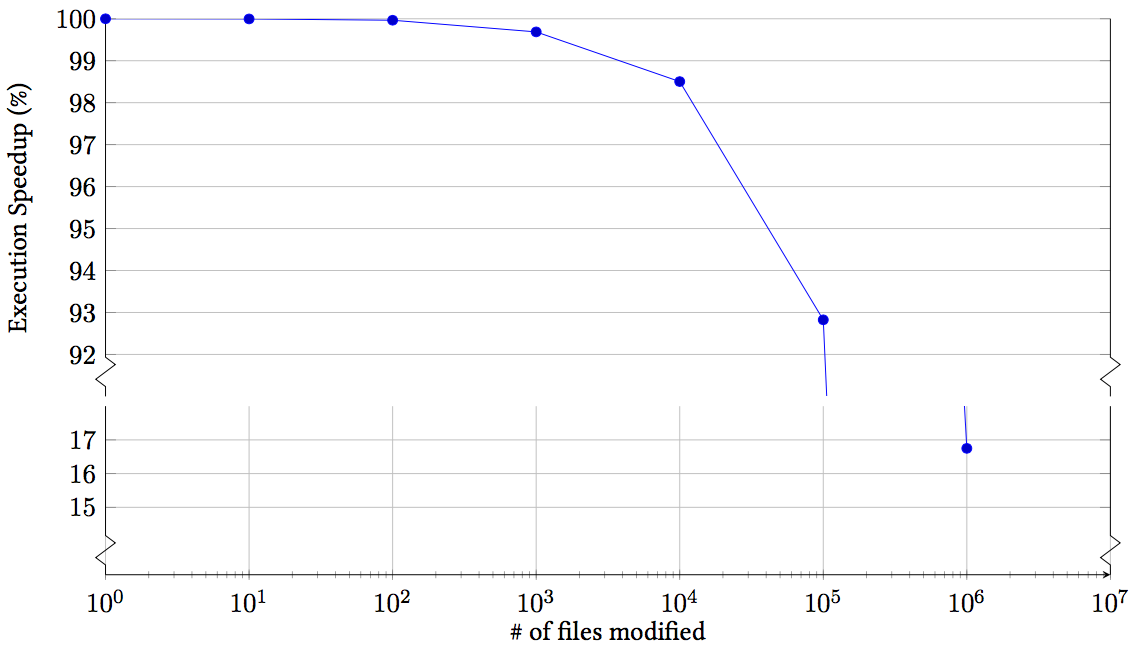
\includegraphics[width=.85\linewidth]{Images/watchdir-mbp.png}
        \end{figure}
  		}
  	\end{tframe}

	\subsection{Local Block Storage}
  	\begin{tframe} \frametitle{Optimisation: Local Block Storage}
  		\only<1>{ \framesubtitle{(i) - Description}
  			\begin{block}<1->{Downloading whole large files for small changes is slow!}
          Implement delta-sync:
          \begin{adv}
            \item Keep a local copy of all files' blocks
            \item Detect what parts of files have been changed
            \item Download only the missing blocks and create the file
          \end{adv}
          \begin{disadv}
            \item Needs extra storage space to store all the different blocks
          \end{disadv}
        \end{block}
        \begin{itemize}
          \item Extend the CloudClient class to handle downloads using blocks.
          \item Use hierarchical structure to improve block lookup speed.
          \item Save local modified blocks after uploads/updates.
        \end{itemize}
  		}
  		\only<2>{ \framesubtitle{(ii) - Sync Process}
  			\begin{figure}[!htpb]
          \centering
          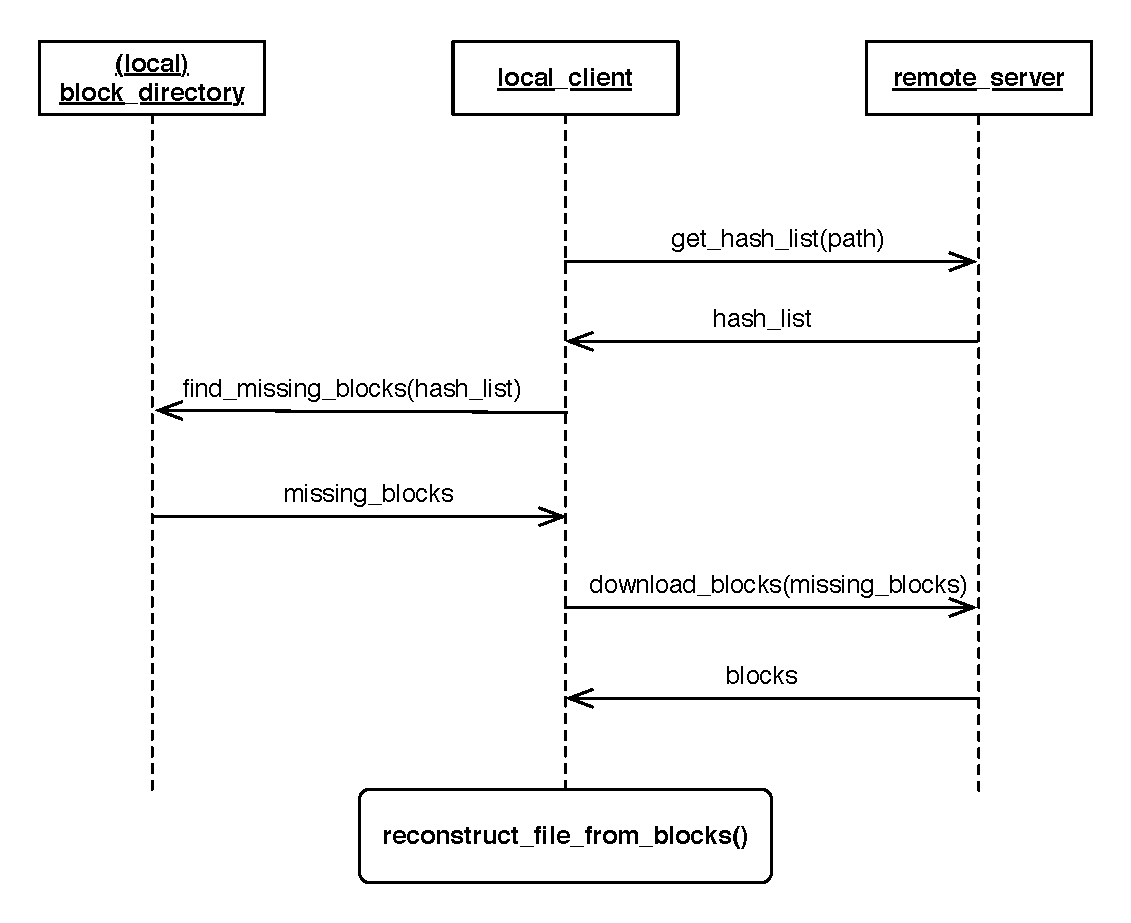
\includegraphics[width=.6\textwidth]{Images/sync_blocks}
        \end{figure}
  		}
      \only<3>{ \framesubtitle{(iii) - Benchmark results}
        \highlightbf{Setup}: Create and upload a 40 MiB (41,943,040 B) file (exactly 10 blocks of 4 MiB), modify some blocks, manually reupload to server, measure download times.
        \begin{table}[!htpb]
          \setlength{\tabcolsep}{12pt}
          \begin{adjustbox}{max width=1.05\textwidth, center}
          \begin{tabular}{c|*{11}{c|}}
            \cline{2-12}
            & \multicolumn{11}{ |c| }{\textbf{\# of modified blocks}}\\ \cline{2-12}
            & \textbf{0} & \textbf{1} & \textbf{2} & \textbf{3} & \textbf{4} & \textbf{5} & \textbf{6} & \textbf{7} & \textbf{8} & \textbf{9} & \multicolumn{1}{|c|}{\textbf{10}}\\ \cline{1-12}
            \multicolumn{1}{|c|}{\textbf{time (s)}} & 0.37 & 2.59 & 4.49 & 6.44 & 8.98 & 10.12 & 12.23 & 13.60 & 15.65 & 17.59 & 19.61 \\ \cline{1-12}
            \multicolumn{1}{|c|}{\textbf{speedup (\%)}} & 98.1 & 86.8 & 77.1 & 67.2 & 54.2 & 48.4 & 37.7 & 30.7 & 20.2 & 10.3 & N/A \\ \cline{1-12}
          \end{tabular}
          \end{adjustbox}
        \end{table}
        \begin{adv}
          \item Linear correlation
          \item Significant improvement for large similar files, since very few blocks need to be downloaded each time
        \end{adv}\\
        \[\textrm{Performance gain \%} = \left(1 - \frac{\textrm{\# of new blocks}}{\textrm{Total \# of blocks}} \right) \times 100\]
      }
      \only<4>{ \framesubtitle{(iv) - Graphical representation}
        \begin{figure}[!htpb]
          \centering
          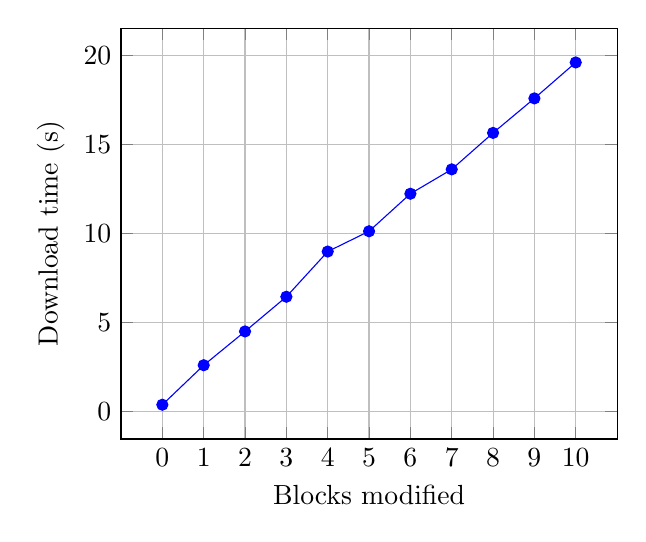
\begin{tikzpicture}
            \begin{axis}[xlabel=Blocks modified, xtick={0,...,10}, ylabel=Download time (s), grid=major, width=0.65\linewidth]
              \addplot[color=blue,mark=*] coordinates {
                (0,0.37) (1,2.59) (2,4.49) (3,6.44) (4,8.98) (5,10.12) (6,12.23) (7,13.60) (8,15.65) (9,17.59) (10,19.61)
              };
            \end{axis}
          \end{tikzpicture}
        \end{figure}
      }
  	\end{tframe}

	\subsection{Local deduplication - FUSE}
		\begin{tframe} \frametitle{Local Deduplication - FUSE}
      \only<1>{ \framesubtitle{(i) - Description}
        % \begin{minipage}{0.48\textwidth}
        \begin{block}<1->{Storing so many large files is expensive!}
          \begin{adv}
            \item Those files have the majority of their blocks in common
            \item We only need to store each block once, in the block directory
            \item Need to control the FS, so we can "virtually" create the files
          \end{adv}
        \end{block}
        \begin{minipage}{0.45\textwidth}
        \highlightbf{Solution}:\\
        Filesystem in Userspace (FUSE) mechanism.
        \end{minipage}
        \begin{minipage}{0.5\textwidth}
        \begin{figure}[!htpb]
          \centering
          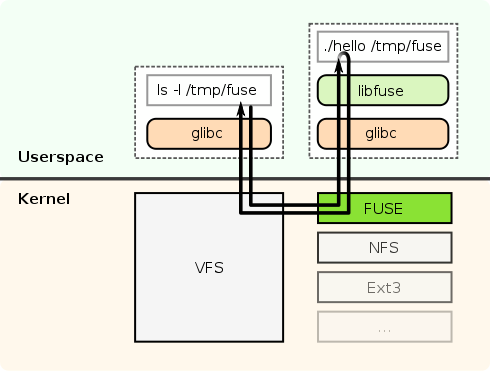
\includegraphics[height=0.45\textheight, width=\textwidth]{Images/FUSE.png}
        \end{figure}
        \end{minipage}
      }
      \only<2>{ \framesubtitle{(ii) - Design}
        \begin{itemize}
          \item Modify \emph{fstat(), open(), read(), write()} system calls to use the blocks a file consists of.
          \item "Write once, Read many, Update never" practice
          \item Copy-on-Write (CoW) strategy, to preserve possibly shared blocks when changes are made
        \end{itemize}
        Effectively implements deduplication on the local file system. Storage space reduction of approximately:
        \small \[block\_size \times \sum_{i=1}^{n}\left[{(\textrm{\# of files sharing block i} - 1}\right]\]
        \normalsize
        Also offers other benefits (cheap file copies, immediate modification detection)
      }
		\end{tframe}

\section{Comparison with existing software}
	\begin{tframe} \frametitle{Comparison with existing software}
	\only<1>{ \framesubtitle{rsync}
    \begin{adv}
      \item Rolling hash algorithm performs exceptionally on detecting modified parts.
      \item Does not need files to be aligned to blocks
      \item One round-trip, works well on high latency connections
      \item Free \& Open source software
    \end{adv}
    \begin{disadv}
      \item Not automated
      \item Needs third-party applications to handle synchronisation
      \item No directory monitoring
      \item Uses MD5 for checksum comparison (potentially unsafe - collisions can be computed)
      \item No local file deduplication
    \end{disadv}
	}
	\only<2>{ \framesubtitle{ownCloud}
		\begin{adv}
      \item Most famous open source synchronisation software suite
      \item Cross-platform
      \item Directory monitoring
    \end{adv}
    \begin{disadv}
      \item {\color{orange-red}No delta-sync - Transfer whole files}
      \item Full local directory scan every few minutes
      \item No local file deduplication
      \item Silently ignores files containing special characters which are not allowed in Windows ('|', ':', '>', '<' and '?')
    \end{disadv}
	}
	\only<3>{ \framesubtitle{Dropbox}
    \begin{adv}
      \item Uses librsync - rolling checksum algorithm benefits
      \item Remote deduplication with blocks of 4 MiB - Fast uploads of similar files
      \item Benchmarks indicated the existance of a local block cache - fast downloads if blocks are cached
      \item Directory Monitoring
      \item Streaming Sync for multiple clients (Prefetching blocks)
    \end{adv}
    \begin{disadv}
      \item Commercial, closed source software
      \item Cannot be deployed on personal cloud storage infrastructures or other cloud storage services
      \item No local file deduplication
    \end{disadv}
	}
	\only<4>{ \framesubtitle{Google Drive}
		\begin{adv}
      \item Directory monitoring
    \end{adv}
    \begin{disadv}
      \item {\color{orange-red}No delta-sync - Transfer whole files}
      \item Commercial, closed source software
      \item Cannot be deployed on personal cloud storage infrastructures or other cloud storage services
      \item No local file deduplication
    \end{disadv}
	}
	\end{tframe}

\section{Future Work}
	\begin{tframe} \frametitle{Future Work}
		\only<1>{ \framesubtitle{ Peer-to-Peer L2 block exchange }
      \highlightbf{Idea:} LAN transfers are faster than over the WAN.\\
      Request missing resources from the LAN, before asking the server.
      \begin{itemize}
        \item Have clients monitor a Link Layer (L2) broadcast address for requests.
        \item Send missing block requests to the network and wait for responses.
        \item When asked, clients check their respective block directories and respond with block availability.
        \item Only request blocks not found in the block directory or the local network from the remote server.
        \item \highlightbf{ALWAYS verify blocks downloaded from LAN} - Avoid corruption or compromise from blocks sent by malicious users.
      \end{itemize}
		}
	\end{tframe}

\begin{tframe} \frametitle{Q \& A}
	Any Questions?
\end{tframe}

\begin{tframe} \frametitle{The End.}
	Thank you for your time!
\end{tframe}

\end{document}